\chapter{Controle de Participação no Projeto}
	
A participação dos estudantes no projeto de extensão universitária foi registrada de forma sistemática, contemplando as tarefas desenvolvidas em cada \textit{sprint}. Esse acompanhamento possibilitou monitorar o cumprimento das atividades propostas e evidenciar tanto o envolvimento do aluno quanto a carga horária dedicada ao projeto. A Tabela~\ref{Tab:TabHoras} apresenta a relação das tarefas executadas, acompanhadas da respectiva descrição, data de realização e número de horas trabalhadas, fornecendo uma visão clara da contribuição efetiva do discente para o desenvolvimento das ações.

\begin{table}[h!]
	\centering
	\caption{Horas Trabalhadas no Projeto.}
	\label{Tab:TabHoras}
	\renewcommand{\arraystretch}{1.3}
	\setlength{\tabcolsep}{8pt}
	\begin{tabular}{c c p{9cm} c}
		\toprule
		\textbf{Sprint} & \textbf{Data} & \textbf{Descrição} & \textbf{Horas} \\
		\midrule
		\multicolumn{3}{l}{\textbf{2024}} & \textbf{107} \\
		\midrule
		\#1 & 30/09/2024 & Task 02 - Modelar o design da tela de abertura do sistema, tela de login e tela administrativa principal. & 15 \\
		\#1 & 30/09/2024 & Task 03 - Modelar design responsivo para telas de celulares. & 12 \\
		\#2 & 13/10/2024 & Task 04 - Definir componentes de acessibilidade. & 30 \\
		\#3 & 26/10/2024 & Task 15 – Criar projeto \textit{front-end React}. & 02 \\
		\#4 & 09/11/2024 & Task 16 – Desenvolver tela de entrada do sistema. & 07 \\
		\#4 & 09/11/2024 & Task 20 – Definir padronização de configurações de acessibilidade e interface. & 09 \\
		\#5 & 23/11/2024 & Task 25 – Desenvolver a tela de cadastro para religião. & 32 \\
		\bottomrule
		\multicolumn{3}{l}{\textbf{2025}} & \textbf{99999} \\
		\midrule
		\#1 &  & Task  - Modelar... . & 15 \\
		\bottomrule
	\end{tabular}
	\legend{Elaborado pelo autor.}
\end{table}
	
\section{Relatório de Sprints}
	
	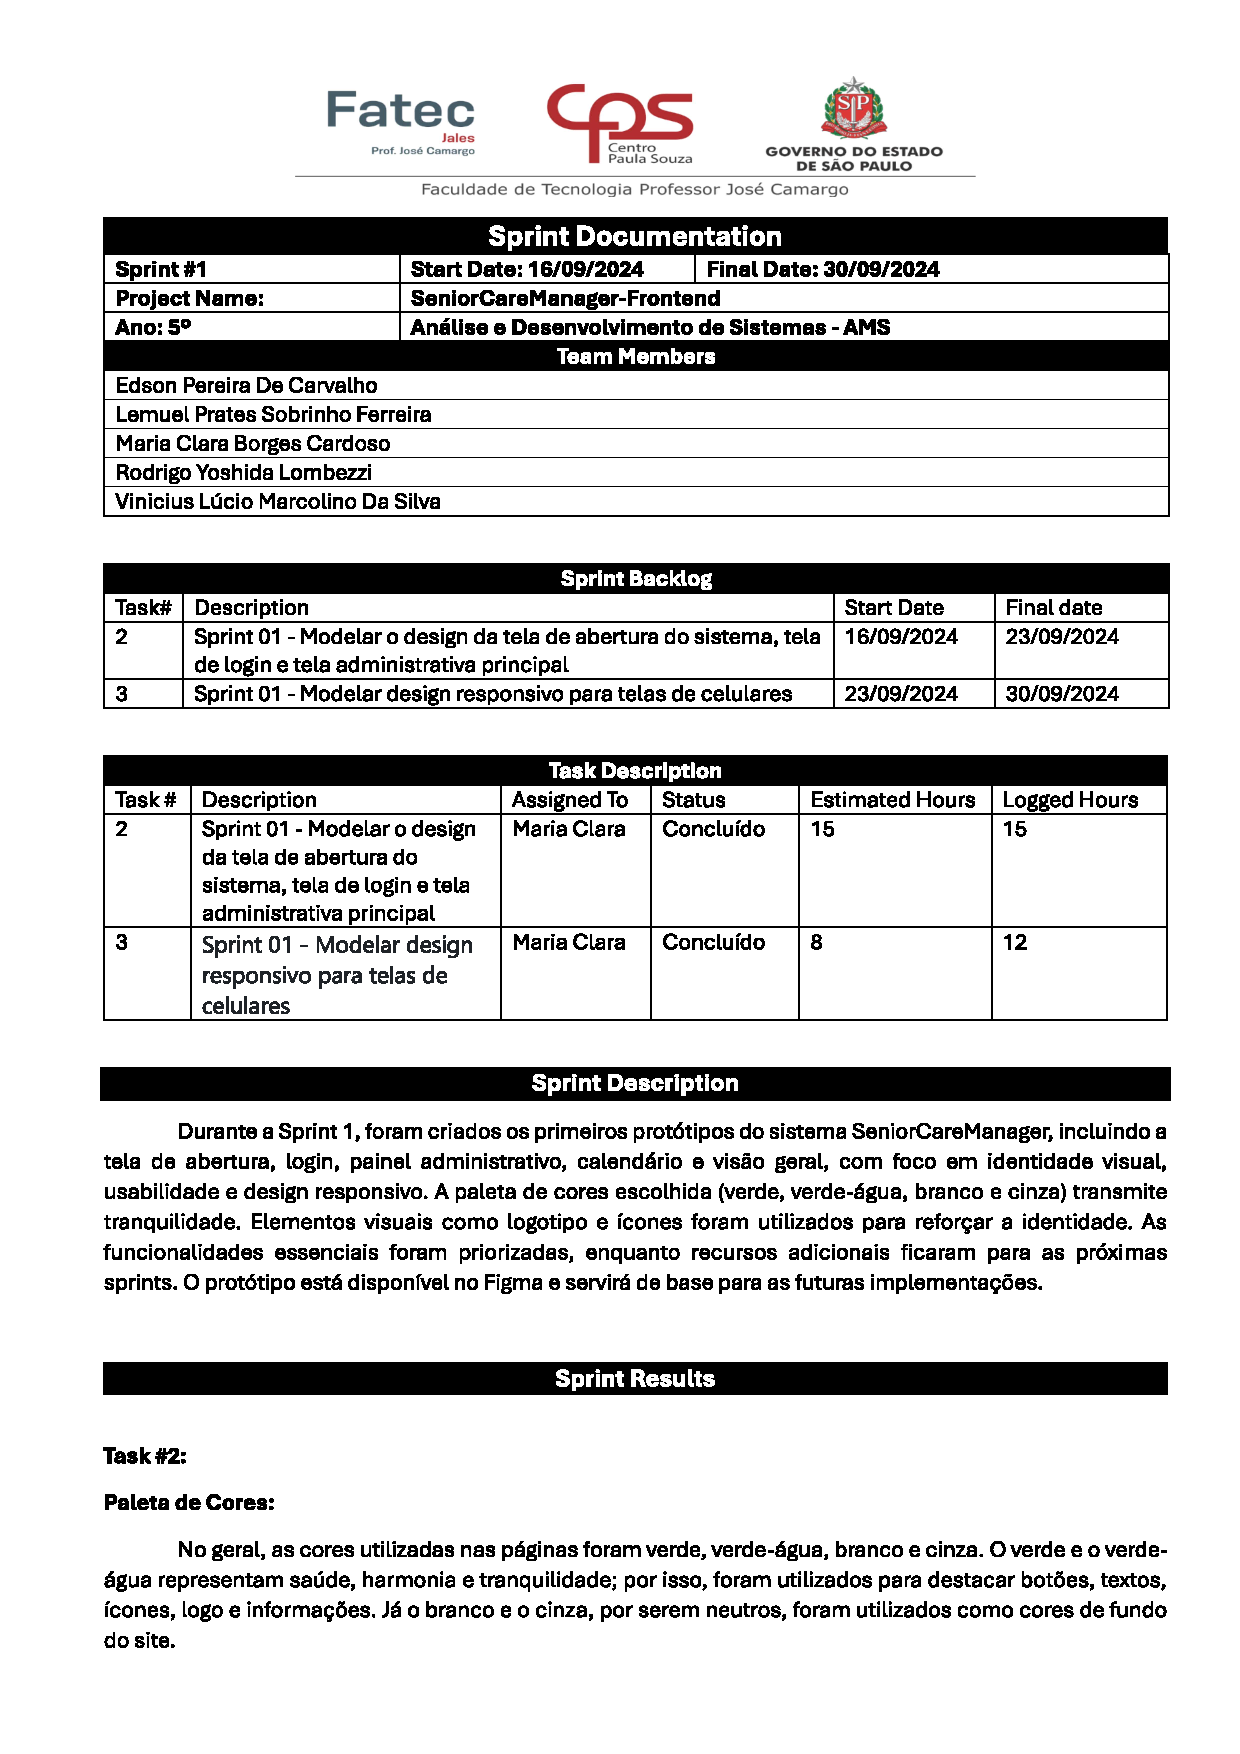
\includepdf[
	scale=0.8,
	pages=1,
	pagecommand={\subsection{Sprint 01 - Task 02 e 03}}
	]{sprints/Sprint01_SeniorCareManager-Frontend_assinado.pdf}
	\includepdf[
	scale=0.8,
	pages=2-14,
	pagecommand={}
	]{sprints/Sprint01_SeniorCareManager-Frontend_assinado.pdf}
	
	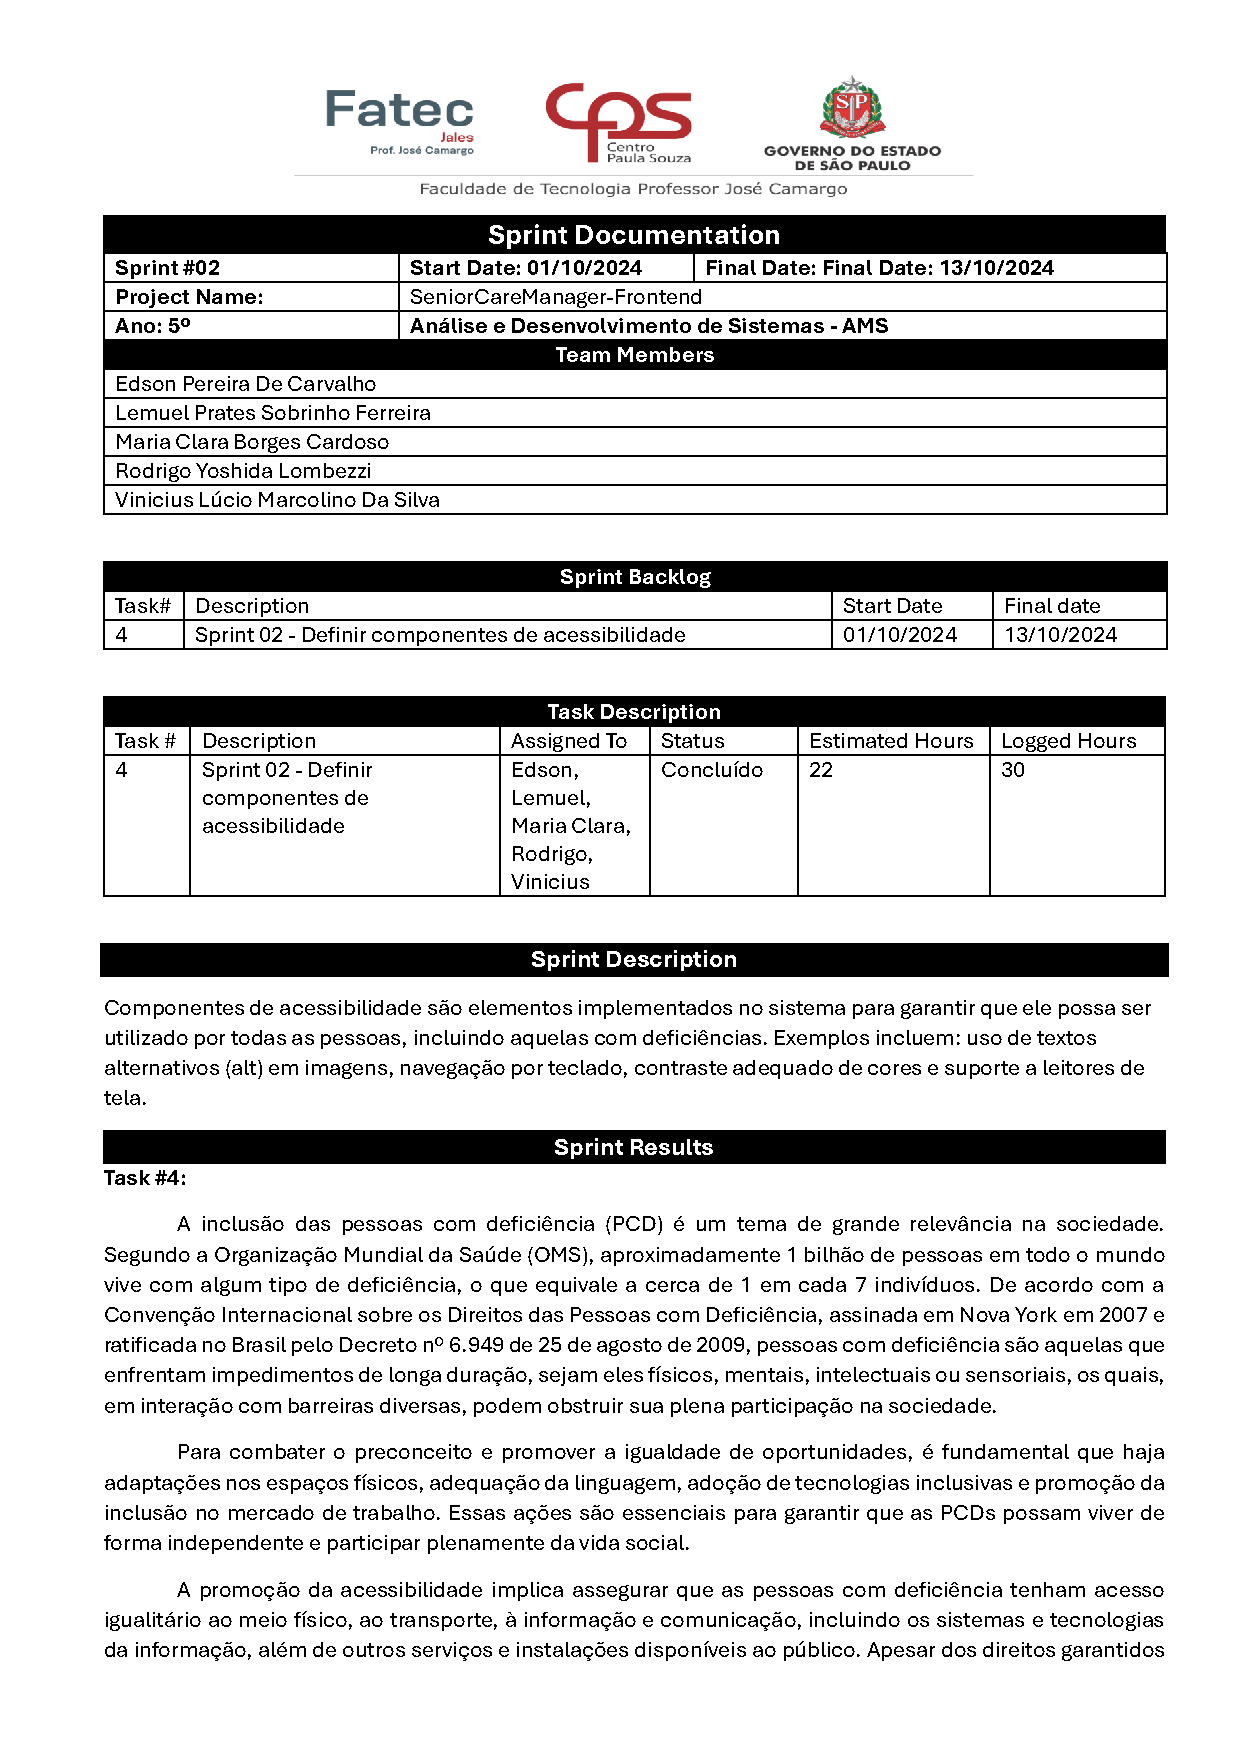
\includepdf[
	scale=0.8,
	pages=1,
	pagecommand={\subsection{Sprint 02 - Task 04}}
	]{sprints/Sprint02_SeniorCareManager-Frontend.pdf}
	\includepdf[
	scale=0.8,
	pages=2-18,
	pagecommand={}
	]{sprints/Sprint02_SeniorCareManager-Frontend.pdf}
	
	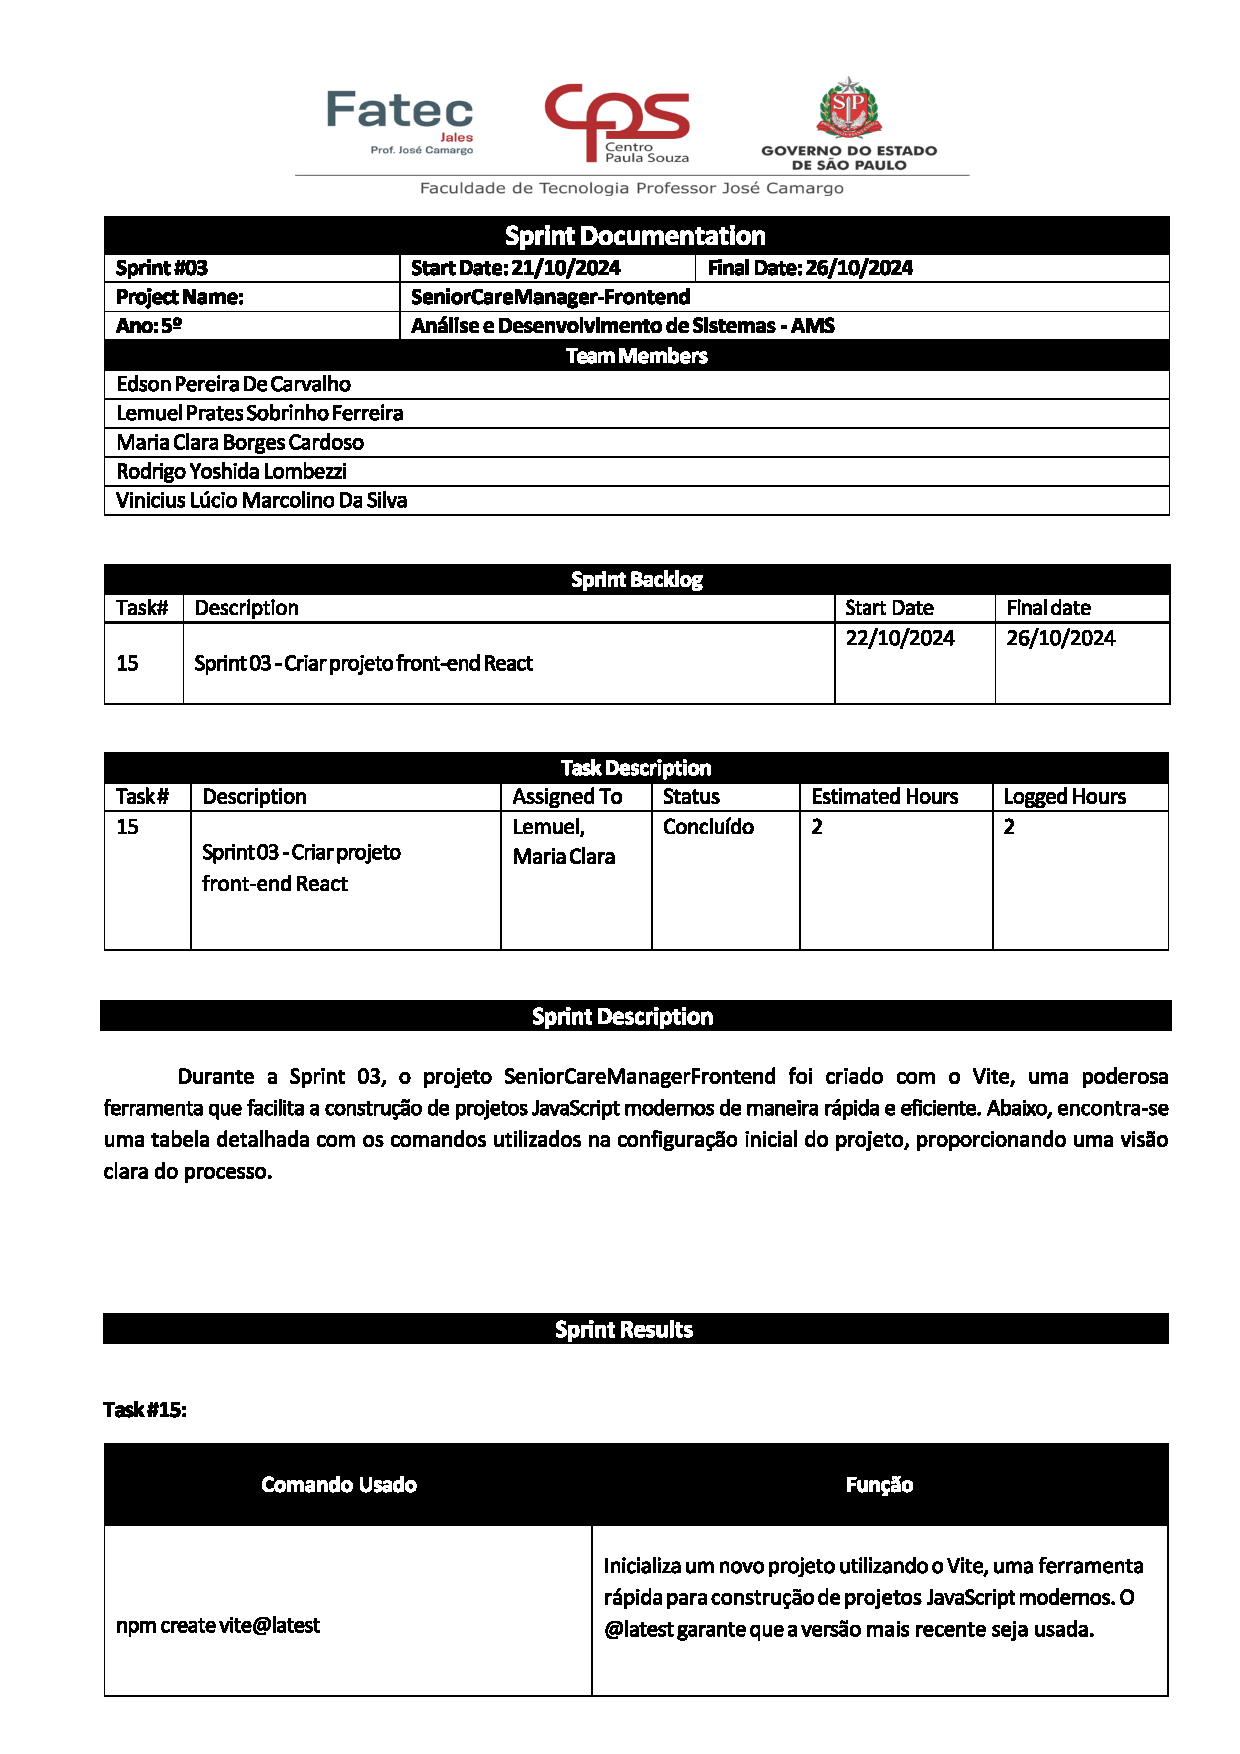
\includepdf[
	scale=0.8,
	pages=1,
	pagecommand={\subsection{Sprint 03 - Task 15}}
	]{sprints/Sprint03_SeniorCareManager-Frontend.pdf}
	\includepdf[
	scale=0.8,
	pages=2,
	pagecommand={}
	]{sprints/Sprint03_SeniorCareManager-Frontend.pdf}
	
	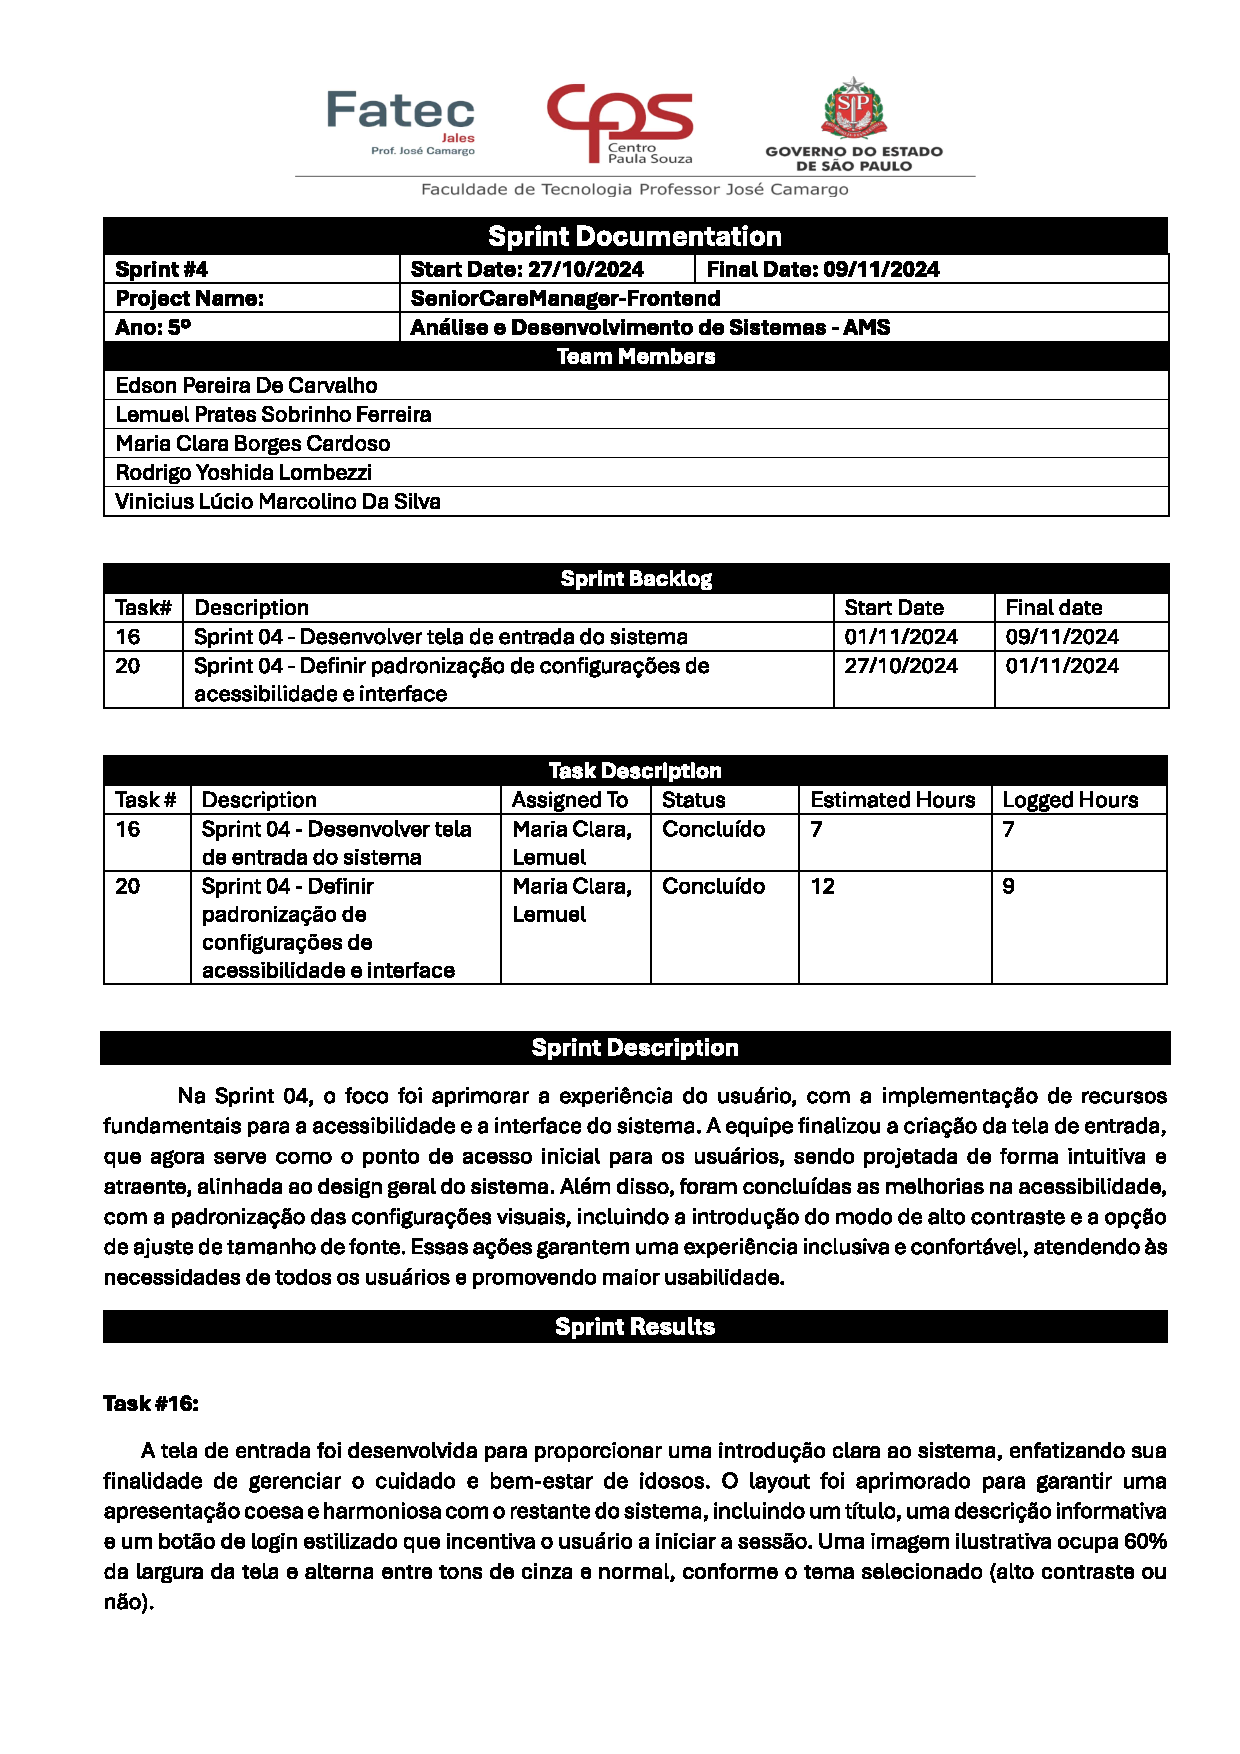
\includepdf[
	scale=0.8,
	pages=1,
	pagecommand={\subsection{Sprint 04 - Task 16 e 20}}
	]{sprints/Sprint04_SeniorCareManager-Frontend.pdf}
	\includepdf[
	scale=0.8,
	pages=2-9,
	pagecommand={}
	]{sprints/Sprint04_SeniorCareManager-Frontend.pdf}
	
	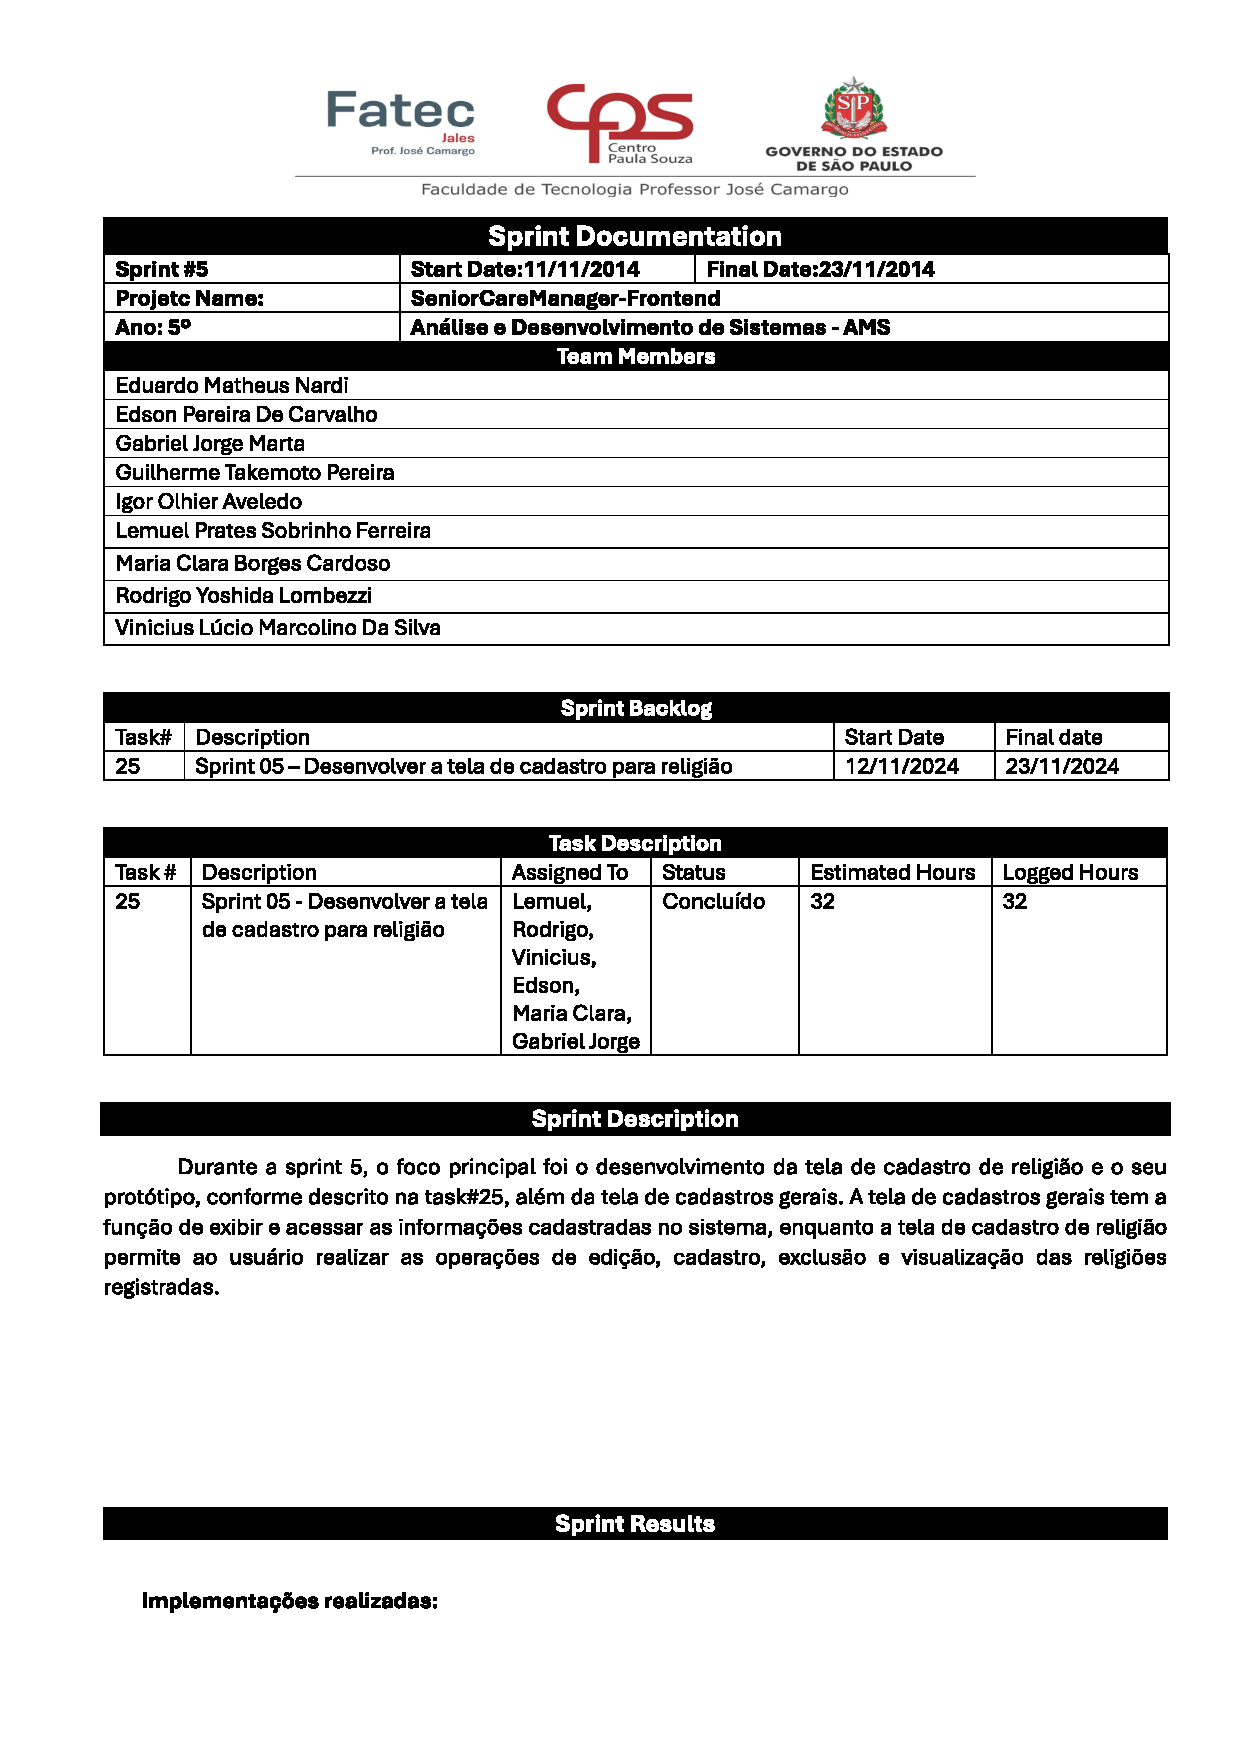
\includepdf[
	scale=0.8,
	pages=1,
	pagecommand={\subsection{Sprint 05 - Task 25}}
	]{sprints/Sprint05_SeniorCareManager-Frontend.pdf}
	\includepdf[
	scale=0.8,
	pages=2-9,
	pagecommand={}
	]{sprints/Sprint05_SeniorCareManager-Frontend.pdf}
